\section{Puzzle zu Listen wandeln} % (fold)
\label{sec:PuzzleToList}
Der Lösungsansatz aus \autocite{Unsolvable-14-15-Numberphile-YT:online} basiert auf Permutationen. Um 4x4 Puzzle besser auf Permutationen untersuchen zu können, werden die Puzzle als Listen von Zahlen dargestellt. Dazu werden die Inhalte der Zellen des Puzzle zeilenweise hintereinander in eine Liste geschrieben. Die Leerstelle, auch als \afz{blank} beschrieben, wird dabei als Zahl \afz{0} interpretiert.
Der Zustand des Puzzle aus Abb.\ref{fig:Perm_puzzle_start_Pic}
\begin{figure}[H]
	\centering
	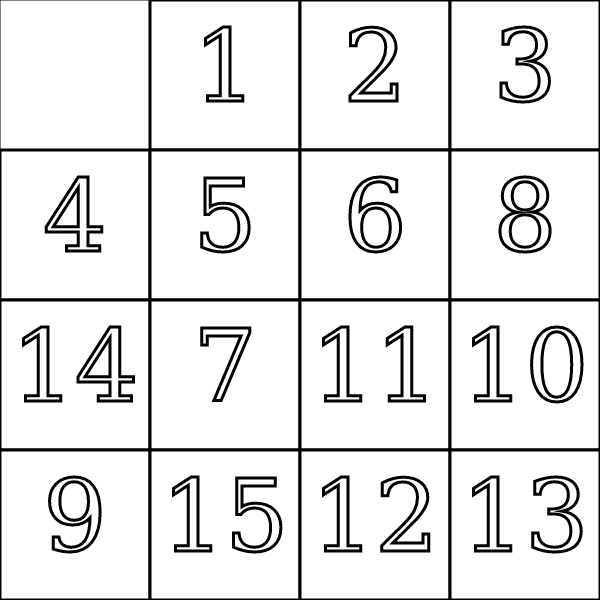
\includegraphics[width=.5\textwidth,keepaspectratio]{img/Start_Puzzle2.png}
	\captionsetup{format=hang}
	\caption{Beispiel Zustand eines 4x4-Puzzle \label{fig:Perm_puzzle_start_Pic}}
\end{figure}
\begin{minipage}{\linewidth}
	wird als Liste aus Zahlen wie folgt dargestellt:
	\begin{center}
		$State = \{0,1,2,3,4,5,6,8,14,7,11,10,9,15,12,13\}$
	\end{center}
\end{minipage}\WNL%
Wichtig ist bei der Betrachtung der lösbaren Puzzle und des Vorgehens der Lösung aus \autocite{Unsolvable-14-15-Numberphile-YT:online} aber auch anderer verfügbarer Quellen \autocite{solving-15-puzzle-lvi:article,geeksforgeeks:online,archer-15-puzzle:article}, dass die Bezeichnung der Leerstelle oder die Art der Konvertierung eines Puzzle zu einer Liste variiert. Die meisten Lösungen sehen den Zielzustand aus Abb.\ref{fig:Perm_puzzle_end_allOther} vor, wobei die Leerstelle dann die Nummer \afz{16} trägt. Um mit den Darstellungen von Herrn Stroetmann aus dem Vorlesungsskript \autocite{github-stroetmann:online} übereinzustimmen, wird der Zielzustand aus Abb.\ref{fig:Perm_puzzle_end_stroet} angestrebt, bei dem die Leerstelle die Nummer \afz{0} trägt.\\
%
\begin{minipage}{\linewidth}
	\begin{minipage}[t]{0.45\linewidth}
		\begin{figure}[H]
			\centering
			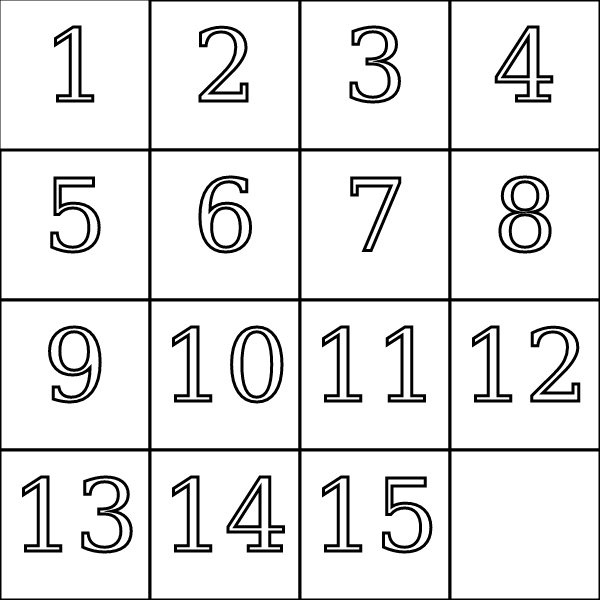
\includegraphics[width=\linewidth,keepaspectratio]{img/End_Puzzle_AO.png}
			\captionsetup{format=plain, indention=0pt}
			\caption{Häufig verwendeter Zielzustand eines 4x4-Puzzle \label{fig:Perm_puzzle_end_allOther}}
		\end{figure}
	\end{minipage}
	\hfill
	\begin{minipage}[t]{0.45\linewidth}
		\begin{figure}[H]
			\centering
			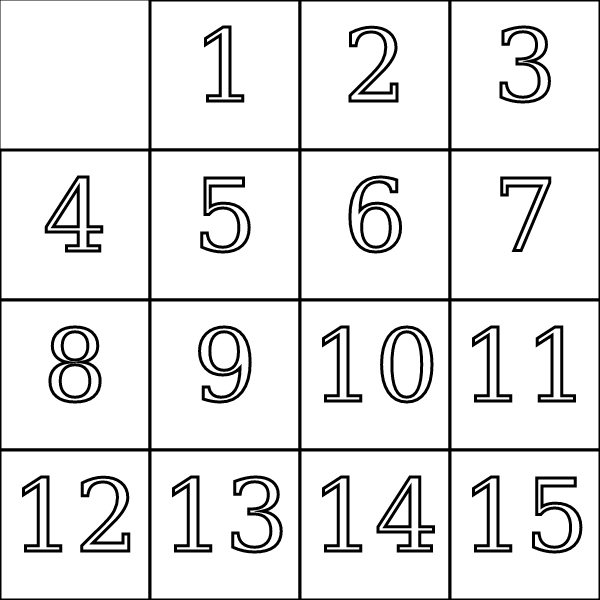
\includegraphics[width=\linewidth,keepaspectratio]{img/End_Puzzle_Stroetmann.png}
			\captionsetup{format=plain, indention=0pt}
			\caption{\label{fig:Perm_puzzle_end_stroet}Verwendeter Zielzustand eines 4x4-Puzzles aus dem Skript von Herrn Stroetmann \autocite{github-stroetmann:online}}
		\end{figure}
	\end{minipage}
\end{minipage}\WNL%
